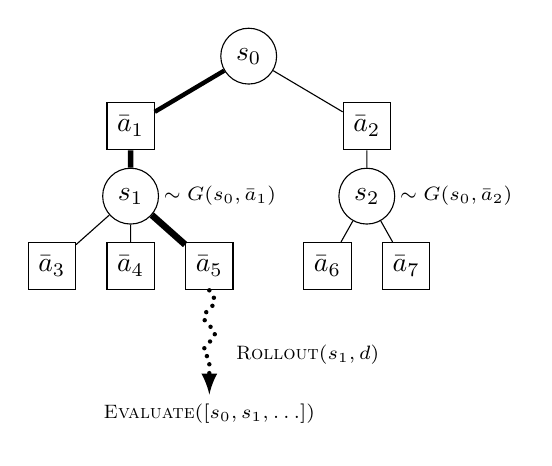
\begin{tikzpicture}[
  nodes={draw, circle}, -, level distance=0.35in,
  every node/.style={circle, draw=black,thin, minimum size = 0.5cm},
  emph1/.style={edge from parent/.style={line width=1.6pt,draw}},
  emph2/.style={edge from parent/.style={line width=2.0pt,draw}},
  emph3/.style={edge from parent/.style={line width=2.4pt,draw}},
  emph4/.style={edge from parent/.style={line width=1.6pt,draw}}, % rollout
  norm/.style={edge from parent/.style={black,thin,draw}},
  evaluate/.style={rectangle, draw=none, minimum height=1mm, edge from parent/.style={black,thin,draw,dotted}},
  action/.style={rectangle, minimum height=6mm, minimum width=6mm},
  evaluate-edge/.style={>=latex, ->, decorate, decoration={snake, amplitude=0.7mm, post length=10pt, segment length=12pt}, dotted, line cap=round, dash pattern=on 0pt off 2\pgflinewidth},
  level 2/.style={sibling distance=10mm},
]
\node{$s_0$}
  child [emph1] { node [norm, action] {$\bar{a}_1$}
    child [emph2] { node [label={[label distance=-1mm]right:{\scriptsize $\sim G(s_0,\bar{a}_1)$}}] {$s_1$}
      child [norm] { node [action] {$\bar{a}_3$} }
      child [norm] { node [action] {$\bar{a}_4$} }
      child [emph3] { node [action] {$\bar{a}_5$}
        child [emph4, level distance=0.74in] { node [evaluate, label={[xshift=1.25cm, yshift=-0.55cm]above:{\scriptsize {\sc Rollout$(s_1,d)$}}}] {\scriptsize {\sc Evaluate$\left([s_0,s_1,\dots]\right)$}}
          edge from parent [evaluate-edge]
        }
      }
    }
  }
  child [norm, missing]
  child [norm] {node [action] {$\bar{a}_2$}
    child [norm] { node [label={[label distance=-1mm]right:{\scriptsize $\sim G(s_0,\bar{a}_2)$}}] {$s_2$} 
      child [norm] { node [action] {$\bar{a}_6$} }
      child [norm] { node [action] {$\bar{a}_7$} }
    }
  };
\end{tikzpicture}